% use paper, or submit
% use 10pt, 11pt or 12pt
% nopagenum removes the page numbers (final conference PDF paper)

\documentclass[paper,11pt]{AAS}
%\documentclass[paper,11pt,nopagenum]{AAS}		% for final proceedings paper version
%\documentclass[submit]{AAS}					% to submit to JAS

\usepackage{bm, tikz, amsmath, overcite, siunitx, graphicx, pgfplots, comment, subcaption}
%\usepackage[notref,notcite]{showkeys}  % use this to temporarily show labels
\usepackage[colorlinks=false, pdfstartview=FitV, linkcolor=red, citecolor=red, urlcolor=red]{hyperref}
\sisetup{output-exponent-marker=\ensuremath{\mathrm{e}}}
\usetikzlibrary{shapes,positioning}
\PaperNumber{24-XXX}

\usepackage{colortbl}
\begin{document}

\title{State Estimation of Chaotic Trajectories:
\\ A Higher-Dimensional, Grid-Based, Bayesian Approach to Uncertainty Propagation}

\author{Benjamin L. Hanson\thanks{Department of Mechanical and Aerospace Engineering, University of California San Diego, La Jolla, CA, 92093, USA.}\ , 
Aaron J. Rosengren\footnotemark[1]\ , and Thomas R. Bewley\footnotemark[1]
}


\maketitle{} 		

\begin{abstract}
    The current landscape of orbital uncertainty propagation methods inadequately addresses the state-estimation problem for nonlinear systems. In relatively low-perturbed regimes, or when measurement updates are frequent, state-estimation methods that assume Gaussian uncertainty are valid, and errors resulting from linearizing the dynamics about an estimate are often negligible. However, as novel space-mission-design techniques exploit the chaoticity of $N$-body dynamics to efficiently explore new regimes of space, the Gaussianity assumption is often violated, and linearization errors accumulate. Uncertainty propagation methods that do not assume Gaussianity or linearize about an estimate are computationally expensive. Moreover, both classes of methods often disregard epistemic uncertainty, or the uncertainty of the model. To address the current limitations of orbital uncertainty propagation, we introduce a higher-dimensional extension to an existing Bayesian-estimation algorithm that efficiently propagates the probability distribution function of a state governed by nonlinear dynamics. By adjusting the computational architecture of the algorithm and considering the dynamics of the system, we scale the existing, three-dimensional technique with poor time complexity to an efficient, four-dimensional one. The result is a robust, second-order accurate, time-adaptive, explicit time-marching scheme with the capability of propagating uncertainty governed by chaotic, nonlinear dynamics. 
\end{abstract}

%\begin{abstract}Grid-based, Bayesian-estimation methods are incredibly useful for state estimation of nonlinear systems when the uncertainty of the state is not necessarily Gaussian. Converse to methods like the ensemble-Kalman Filter, these full-Bayesian-estimation techniques propagate the entirety of the probability-density function (PDF), rather than just the mean and higher-order moments. Due to the extensive nature of the strategy with respect to memory, scaling to higher dimensions becomes computationally impractical. By adjusting the architecture of the algorithm and preserving the physical nature of the system, we scale a grid-based Bayesian estimation method to 4, 5, and 6 dimensional cases with ease. To improve the efficiency of state estimation and propagation in astrodynamical systems, we utilize a slow-moving coordinate frame, where the majority of the variables stay ``linear'' for longer. This extension to higher dimensions allows us to examine and quantify more complicated systems, such as the astrodynamics of a satellite in a chaotic orbit. 
%\end{abstract}

\section{Introduction}

Since the dawn of space exploration, orbital uncertainty propagation has seen relatively little change. Much of the success of the Apollo lunar missions can be attributed to the work of Kalman, specifically the extended-Kalman filter\cite{kalman} (EKF), the primary algorithm used by on-board systems that determined accurate state estimates of the Apollo spacecraft\cite{sF81}. This foundational algorithm ensured the feasibility of the complex trajectories essential to the Apollo lunar missions. Since the Space Race, spaceflight has undergone a complete upheaval in almost all facets. Advances in additive manufacturing have resulted in fully 3D-printed rocket engines and propellant tanks that are more weight- and cost-efficient than their legacy counterparts\cite{eS22, rC14}. Low-thrust relative transfers have motivated the creation of novel low-thrust propulsion methods, such as ionic propulsion\cite{jB03} and solar-sail systems\cite{yT13}. There are numerous domains of spaceflight that are almost unrecognizable when compared with their ancestral systems. Conversely, one of the most recent NASA missions, Artemis-1, employed the Orion Absolute Navigation System that utilized four navigation EKFs for estimating the vehicle's state and associated uncertainty\cite{jS23}, the same framework used in the Apollo missions over 60 years ago. In a field where rapid growth is the norm, this sort of stagnation is unprecedented. 

By no means is the prior paragraph meant to discredit the EKF. On the contrary, its persistent utilization over the last several decades in the fields of orbit determination, conjunction analysis, guidance, navigation, and control (GN\&C), space situational awareness (SSA), etc., serves as a testament to its robustness. However, there are limitations to this robustness. For instance, the EKF approximates the dynamics of a nonlinear system by linearizing about an estimate. This linearization can result in the EKF underestimating uncertainty and depending heavily on precise initial estimates. Additionally, the EKF assumes the uncertainty of an object may be described by a multivariate Gaussian distribution. In the absence of measurement updates, this holds for a period of time, but the length of this period is dependent on the dynamics of the system. Both of these limitations are predicated on the assumption that the measurement update frequency will be high enough that the errors associated with linearizing are negligible and the state uncertainty stays Gaussian. However, the validity of this assumption is brought into question in the presence of chaotic dynamics, as is the case when the motion of an object with negligible mass is governed by two massive bodies, known as the restricted three-body problem (R3BP)\cite{jG97}. Novel space-mission-design techniques aim to exploit the chaoticity of three- and four-body dynamics via new families of low-energy trajectories that are more fuel efficient, longer in duration, and further in reach than their classical counterparts\cite{sR22}. CAPSTONE, a CubeSat pathfinder for the Lunar Gateway and a cornerstone of NASA's Artemis Program, utilized a low-energy, ballistic lunar transfer\cite{parker_thesis} (BLT), a family of these low-energy transfers, to insert into its operational near-rectilinear halo orbit (NRHO) about the $L_2$ Earth-Moon libration point in November of 2022\cite{mT21}. Future proposed missions to the Jovian and Saturnian moons \cite{sR22, sC13} are expected to utilize the $N$-body dynamics of the respective systems for low-energy trajectory design. As the standard for mission complexity increases to incorporate these novel trajectory designs, so too does the necessity for effective state-estimation and uncertainty propagation techniques that address the limitations of the EKF and provide more precise solutions in these chaotic regimes. 

There are other uncertainty propagation methods that attempt to address the shortcomings of the EKF, each with their own limitations. Monte-Carlo (MC) simulations, for instance, circumvent the assumption of Gaussianity by generating $N$ random samples, called \textit{particles}, from the initial uncertainty. The state of these particles are then time-marched, governed by the dynamics of the system \cite{yL17}. As $N\rightarrow \infty$, the final distribution of the samples approaches the true probability distribution. However, obtaining this true distribution requires an unknown-but-significant number of samples, and, in especially chaotic regimes that are extremely sensitive to initial conditions, achieving this number may be computationally expensive. Additionally, current MC methods cannot viably consider epistemic uncertainty \cite{TR15}, the uncertainty of the model, an important consideration for unexplored, chaotic regimes. Another family of techniques that attempts to rectify the limitations of the EKF are Gaussian-mixture models\cite{yL17} (GMMs). GMMs approximate an arbitrary PDF as a collection of weighted Gaussian distributions, then propagate the mean and covariance of each of the distributions in the collection. However, when the true probability distribution ``bananas'' about a nominal trajectory, as has been demonstrated for nonlinear systems \cite{kF12}, many Gaussian distributions are necessary for representing the true distribution, leading to a computational bottleneck. Additionally, determining and updating the weights of the Gaussian mixtures, as well the splitting procedure, can be both expensive and ad hoc.

In summary, having performed a preliminary review of the landscape of methods that represent and propagate orbital uncertainty, we have determined that there exists a need for a new class of methods that do not assume Gaussian uncertainty, are accurate for long periods of time in the absence of observations, are computationally efficient, consider epistemic uncertainty, and are scalable to higher-dimensional problems. To address this need, we propose an astrodynamical extension to an existing nonlinear, state-estimation method known as Grid-based, Bayesian estimation exploiting sparsity\cite{tB12} (GBEES). GBEES efficiently solves the Fokker-Planck equation (FPE), which describes the time-evolution of a PDF governed by nonlinear dynamics. Bayesian estimation strategies are foundational in the way they address the state estimation problem, but have often been disregarded due to their computational inefficiency \cite{mA02}. GBEES addresses this issue by considering the sparsity of a PDF over the majority of phase space, thereby cutting down on the computational expense of numerically solving the FPE over a large grid. However, the legacy implementation is susceptible to computational burden at higher dimensions given its $\mathcal{O}(n^2)$ time complexity (where $n$ is the number of grid cells that make up the discretized PDF), making it sub-optimal for orbital uncertainty propagation. The extension we propose reduces this time complexity via efficient data structures and a consideration of the dynamics of the system. We demonstrate the method on a 4D astrodynamical system, and layout the possibility for expanding to higher-fidelity models. 

\section{Grid-Based, Bayesian Estimation Exploiting Sparsity}

To ensure full understanding of the proposed extension, we provide a succinct explanation of the parent algorithm, GBEES (a complete explanation is included in Ref.~\citenum{tB12}). Consider the state estimation of a nonlinear system
\begin{gather}\label{eq:NLsystem}
    \frac{d\mathbf{x}}{dt} = \mathbf{f}(\mathbf{x},\mathbf{w}), \quad \mathbf{y} = \mathbf{h(\mathbf{x}, \mathbf{v}}),
\end{gather}
\noindent where $\mathbf{x}$ is the state of the system, $\mathbf{f}(\cdot)$ is the nonlinear system function, $\mathbf{w}$ is the state disturbance, $\mathbf{y}$ is the measurement of the system, $\mathbf{h}(\cdot)$ is the measurement function, and $\mathbf{v}$ is the measurement noise. The evolution of the PDF $p_\mathbf{x}(\mathbf{x}',t)$ of the state $\mathbf{x}$ is performed via mixed continuous/discrete time-marching \cite{aJ70} and can be described in two steps:

\begin{enumerate}
    \item Between discrete measurements, $p_\mathbf{x}(\mathbf{x}',t)$ is marched via discretization of the Fokker-Planck equation \cite{aF14,mP17}(FPE); in Einstein-summation notation: 
    \begin{subequations}
    \begin{gather}\label{eq:FPE}
        \frac{\partial p_\mathbf{x}(\mathbf{x}',t)}{\partial t} = -\frac{\partial f_i(\mathbf{x}',t)p_\mathbf{x}(\mathbf{x}',t)}{\partial x_i'} + \frac{1}{2}\frac{\partial^2q_{ij}p_\mathbf{x}(\mathbf{x}',t)}{\partial x_i'x_j'},
    \end{gather} 
    where $q_{ij}$ is the $(i,j)$th element of the spectral density of the state disturbances, $Q$. When $Q=0$, the PDE is hyperbolic. 
    \item At measurement interval $t_k$, $p_\mathbf{x}(\mathbf{x}',t)$ is updated via Bayes' Theorem \cite{tB63}:
    \begin{gather}\label{eq:Bayes}
        p_\mathbf{x}(\mathbf{x}',t_{k+}) = \frac{p_\mathbf{y}(\mathbf{y}_k|\mathbf{x}')p_\mathbf{x}(\mathbf{x}',t_{k-})}{C},
    \end{gather}
    \end{subequations}
    where $p_\mathbf{x}(\mathbf{x}',t_{k+})$ is the \textit{a posteriori} PDF, $p_\mathbf{y}(\mathbf{y}_k|\mathbf{x}')$ is the distribution associated with the measurement, $p_\mathbf{x}(\mathbf{x}',t_{k-})$ is the \textit{a priori} PDF, and $C$ is a normalization constant. 
\end{enumerate}
To discretize the hyperbolic form of Eq.~\eqref{eq:FPE} (i.e. when $Q=0$), a Godunov-type, finite-volume method \cite{rL07} is utilized. In 2D (with higher-dimensional cases following as obvious extensions), this takes the form 
\begin{equation}\label{eq:FPE_discretized}
    \frac{p_{ij}^{n+1}-p_{ij}^n}{\Delta t} = - \frac{F_{i+1/2,j}^n-F_{i-1/2,j}^n}{\Delta x} - \frac{G_{i,j+1/2}^n-G_{i,j-1/2}}{\Delta y},
\end{equation}
where $n$ represents the time step, $\Delta x$ and $\Delta y$ are the grid widths in the $x$- and $y$-directions respectively, $p_{ij}$ is the probability at grid cell $(i,j)$, and fluxes $F$ and $G$ are defined at the interfaces of the grid, thus the half-step indexing. The resulting grid of Riemann problems are solved numerically at the interfaces of each grid cell for every time step. Accounting for \textit{corner-transport upwind} and \textit{flux-limiting} corrections, the result is an explicit, $2^{\textrm{nd}}$-order accurate, time-marching scheme that propagates the PDF governed by the dynamics of the system $\mathbf{f}(\mathbf{x})$. To save on computational cost, the algorithm only accounts for grid cells that have a probability above some threshold $\bar{p}$, thoroughly lessening the number of operations necessary for each time step. As the probability flows throughout phase space, new cells are inserted about those who have surpassed the probability threshold, and cells below $\bar{p}$ without such neighbors are deleted. Thus, most of the PDF is represented with a small percentage of the domain of phase space. 

For validation, the GBEES algorithm is demonstrated on a 3D Lorenz attractor \cite{eL63}, a highly chaotic solution set to the Lorenz system. In this system, uncertainty quickly transforms from Gaussian to non-Gaussian. For the 3D Lorenz system 
\begin{gather}\label{eq:Lorenz}
   \mathbf{x} = \begin{bmatrix}
       x \\ y \\ z
   \end{bmatrix}, \quad \frac{d\mathbf{x}}{dt} = \mathbf{f}(\mathbf{x}) = \begin{bmatrix}
       \sigma (y - x) \\ -y-xz \\ -bz+xy-br
   \end{bmatrix}, 
\end{gather}
with parameter values $\sigma = 4$, $b=1$, and $r=48$ resulting in a chaotic system. Figure~\ref{fig:3DLorenz} depicts the chaotic dynamics governing the system, as well as the continuous time-evolution of an initially Gaussian PDF in the absence of discrete measurements, with $Q=0$ (assuming no uncertainty of the system). 
\begin{figure}[htb]
    \centering\includegraphics[width=0.49\textwidth]{Figures/Lorenz3D/GBEES.eps}\hspace{-0.4 cm}
    \centering\includegraphics[width=0.49\textwidth]{Figures/Lorenz3D/GBEES_MC.eps}
    \caption{The continuous time-evolution of an initially Gaussian PDF with no discrete measurement updates. ({\it right}) The PDF is described by the {\it blue isosurfaces} of probability $p=\num{5e-3}$, $p=\num{5e-4}$, and $p=\num{5e-5}$ at times $t=0$, $t=0.2$, $t=0.4$, $t=0.6$, $t=0.8$, and $t=1$. The {\it green line} represents the Lorenz attractor, the dynamics of which govern the flow of probability. The {\it black line} represents the nominal trajectory, about which the initial uncertainty is estimated. ({\it left}) The outermost {\it isosurface} ($p=\num{5e-5}$) compared to a 1000 particle Monte-Carlo simulation with the same initial conditions, represented by the {\it gray} trajectories and {\it black dots}. A complete list of the simulation parameters can be found in Table~\ref{tab:GBEES_parameters}.}
    \label{fig:3DLorenz}
\end{figure}
As can be seen, the Gaussian distribution quickly becomes non-Gaussian, and even becomes bimodal near $t=1$, a characteristic that is indescribable by the EKF. The right subfigure of Figure~\ref{fig:3DLorenz} demonstrates that the outermost isosurface ($p=\num{5e-5}$) of the PDF propagated by GBEES captures the results of the Monte-Carlo simulation starting with the same initial conditions and covariance. Due to its extreme nonlinearity, describing the final PDF using a GMM would require a computationally expensive number of Gaussian distributions. 

\section{Addressing the $\mathcal{O}(n^2)$ time complexity}

The primary issue with the legacy GBEES implementation arises as we push towards higher dimensions. Scaling to higher-dimensional systems requires discretizing a larger domain of phase space, leading to increases in the number of cells needed to represent a PDF. As cells are created and deleted based on the probability threshold constraint, neighboring cells must be adjusted to consider the information provided by the new discretization. In the legacy implementation, said adjustments are performed through nested loops, leading to a time complexity of $\mathcal{O}(n^2)$ for the entire algorithm, resulting in the inefficiency at higher dimensions. The aim of the proposed extension is to eliminate this computational bottleneck, as well as look for subprocedures that can be made more efficient. As this is a computational limitation, the following discussion is over the modifications and adjustments implemented to optimize the algorithm's architecture.

\subsection{Binary Search Trees}

Bayesian-estimation methods are predicated on the ability to efficiently perform the grid updates associated with time-marching the numerical solution to Eq.~\eqref{eq:FPE}. As such, utilizing efficient data structures within the chosen finite volume method is of the utmost importance. The legacy implementation of GBEES stores the discretized Cartesian grid in a list, which has an $\mathcal{O}(n)$ time complexity for creation, deletion, and searching. As the algorithm countlessly uses all three of these procedures throughout, improving their individual time complexities is greatly beneficial. One such data structure that has a better time complexity ($\mathcal{O}(\log n)$ for creation, deletion, and searching) are binary search trees (BSTs). 

\paragraph{Introduction to BSTs.} 

BSTs \cite{BST} sort data using a positive-integer key $z$. Each datum, known as a \textit{node}, stores its own key value as well as pointers to the left and right \textit{child nodes}. The left child has a value $z$ less than the parent node, and the right child has a value $z$ greater than the parent node. Searching a BST to see if a key exists begins by comparing the key being searched for to the \textit{root node}, or the first node in the tree. The search then traverses left or right down the tree, depending on if the key being searched for is less than or greater than the root node, respectively. This process is repeated until the key being search for is reached, or a \textit{leaf node} is reached (a node with no left or right child). In this case, the key being searched for does not exist in the BST. Creation and deletion of nodes follow in similar fashions.

\begin{comment}
\begin{figure}[htb]
  \centering
  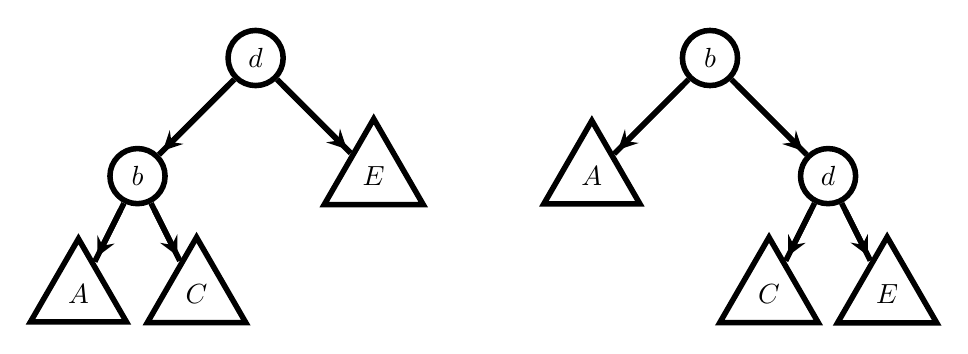
\begin{tikzpicture}[
    level/.style={sibling distance=30mm/#1, line width=2pt},
    circleNode/.style={circle, draw, minimum size=7mm, line width=2pt},
    triangleNode/.style={regular polygon, regular polygon sides=3, draw, minimum size=7mm, line width=2pt},
    arrow/.style={->, >=stealth, shorten >= 2pt, shorten <= 3pt, line width=2pt}
  ]

  % First Tree
  \node[circleNode] (root1) {$d$}
    child {node[circleNode] (node1) {$b$}
      child {node[triangleNode] (node2) {$A$}}
      child {node[triangleNode] (node3) {$C$}}
    }
    child {node[triangleNode] (node4) {$E$}
    };

  % Arrows
  \draw[arrow, line width=2pt] (root1) -- (node1);
  \draw[arrow, line width=2pt] (root1) -- (node4);
  \draw[arrow, line width=2pt] (node1) -- (node2);
  \draw[arrow, line width=2pt] (node1) -- (node3);

  % Second Tree
  \node[circleNode, right=5cm of root1] (root2) {$b$}
    child {node[triangleNode] (node6) {$A$}
    }
    child {node[circleNode] (node9) {$d$}
      child {node[triangleNode] (node10) {$C$}}
      child {node[triangleNode] (node11) {$E$}}
    };

  % Arrows
  \draw[arrow, line width=2pt] (root2) -- (node6);
  \draw[arrow, line width=2pt] (root2) -- (node9);
  \draw[arrow, line width=2pt] (node9) -- (node10);
  \draw[arrow, line width=2pt] (node9) -- (node11);

  \end{tikzpicture}
  \caption{Two equivalent BSTs, where the left can be transformed into the right via a \textit{right rotation}, and the right can be transformed into the left via a \textit{left rotation}. Each letter represents the key value, thus $A < b < C < d < E$. Triangle nodes represent nodes that are themselves BSTs.}
  \label{fig:BST}
\end{figure}
  \begin{figure}[htb]
  \centering
  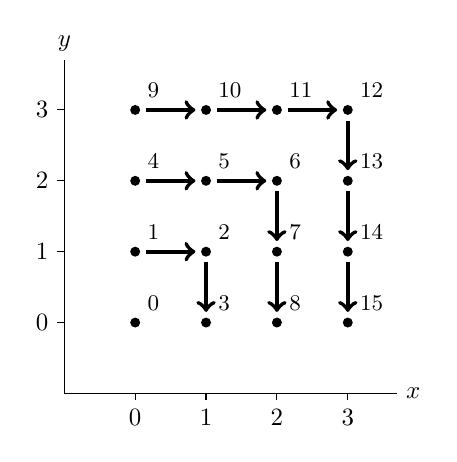
\begin{tikzpicture}[scale=0.9, transform shape]
    % Draw axes with an offset
    \draw[-] (-1,-1) -- (3.7,-1) node[right] {$x$};
    \draw[-] (-1,-1) -- (-1,3.7) node[above] {$y$};

    % Draw grid
    \foreach \x in {0,1,2,3}
      \draw (\x,-1) -- (\x,-1.1) node[below] {\x};
    \foreach \y in {0,1,2,3}
      \draw (-1,\y) -- (-1.1,\y) node[left] {\y};

    % Draw dots at each coordinate point
    \foreach \x in {0,1,2,3}
      \foreach \y in {0,1,2,3}
        \pgfmathtruncatemacro{\RS}{max(\x,\y)^2+max(\x,\y)+\x-
        \y}
        \fill (\x,\y) circle (2pt) node[anchor=south west, font=\fontsize{9}{12}\selectfont] at (\x+0.05,\y+0.05) {\RS};

    % Draw hor. connecting arrows
    \draw[->, line width=1.5pt] (0.15,1) -- (0.85,1);
    \draw[->, line width=1.5pt] (0.15,2) -- (0.85,2);
    \draw[->, line width=1.5pt] (0.15,3) -- (0.85,3);
    \draw[->, line width=1.5pt] (1.15,2) -- (1.85,2);
    \draw[->, line width=1.5pt] (1.15,3) -- (1.85,3);
    \draw[->, line width=1.5pt] (2.15,3) -- (2.85,3);

    % Draw ver. connecting arrows
    \draw[->, line width=1.5pt] (1,0.85) -- (1,0.15);
    \draw[->, line width=1.5pt] (2,0.85) -- (2,0.15);
    \draw[->, line width=1.5pt] (3,0.85) -- (3,0.15);
    \draw[->, line width=1.5pt] (2,1.85) -- (2,1.15);
    \draw[->, line width=1.5pt] (3,1.85) -- (3,1.15);
    \draw[->, line width=1.5pt] (3,2.85) -- (3,2.15);

  \end{tikzpicture}
  \caption{RS pairing in two dimensions.}
  \label{fig:RS_pairing}
\end{figure}    
\end{comment}

\begin{figure}
    \begin{minipage}{0.575\textwidth}
        \centering
        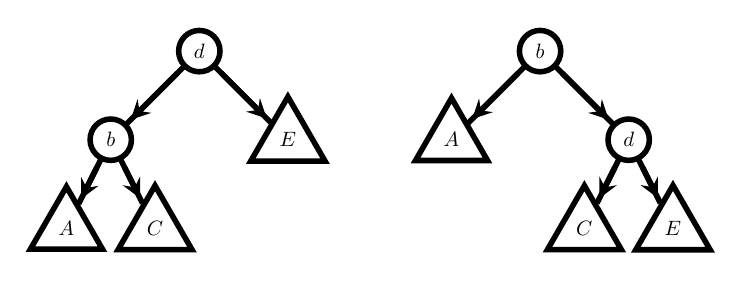
\begin{tikzpicture}[
    level/.style={sibling distance=30mm/#1, line width=2pt},
    circleNode/.style={circle, draw, minimum size=7mm, line width=2pt},
    triangleNode/.style={regular polygon, regular polygon sides=3, draw, minimum size=7mm, line width=2pt},
    arrow/.style={->, >=stealth, shorten >= 2pt, shorten <= 3pt, line width=2pt},
  scale=0.75, transform shape]

  % First Tree
  \node[circleNode] (root1) {$d$}
    child {node[circleNode] (node1) {$b$}
      child {node[triangleNode] (node2) {$A$}}
      child {node[triangleNode] (node3) {$C$}}
    }
    child {node[triangleNode] (node4) {$E$}
    };

  % Arrows
  \draw[arrow, line width=2pt] (root1) -- (node1);
  \draw[arrow, line width=2pt] (root1) -- (node4);
  \draw[arrow, line width=2pt] (node1) -- (node2);
  \draw[arrow, line width=2pt] (node1) -- (node3);

  % Second Tree
  \node[circleNode, right=5cm of root1] (root2) {$b$}
    child {node[triangleNode] (node6) {$A$}
    }
    child {node[circleNode] (node9) {$d$}
      child {node[triangleNode] (node10) {$C$}}
      child {node[triangleNode] (node11) {$E$}}
    };

  % Arrows
  \draw[arrow, line width=2pt] (root2) -- (node6);
  \draw[arrow, line width=2pt] (root2) -- (node9);
  \draw[arrow, line width=2pt] (node9) -- (node10);
  \draw[arrow, line width=2pt] (node9) -- (node11);

  \end{tikzpicture}
        \caption{Two equivalent BSTs, where the {\it left} can be transformed into the {\it right} via a \textit{right rotation}, and the {\it right} can be transformed into the {\it left} via a \textit{left rotation}. Each letter represents the key value, thus $A < b < C < d < E$. Triangle nodes represent nodes that are themselves BSTs.}
        \label{fig:BST}
    \end{minipage}
    \hfill
    \begin{minipage}{0.375\textwidth}
        \centering
         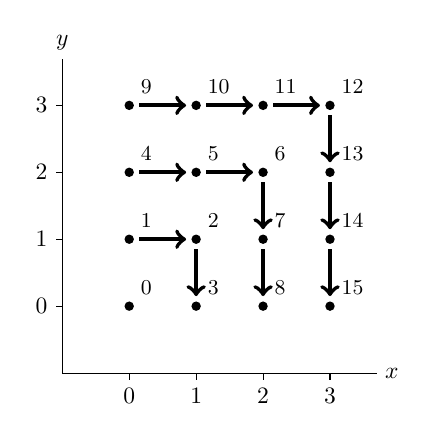
\begin{tikzpicture}[scale=0.85, transform shape]
    % Draw axes with an offset
    \draw[-] (-1,-1) -- (3.7,-1) node[right] {$x$};
    \draw[-] (-1,-1) -- (-1,3.7) node[above] {$y$};

    % Draw grid
    \foreach \x in {0,1,2,3}
      \draw (\x,-1) -- (\x,-1.1) node[below] {\x};
    \foreach \y in {0,1,2,3}
      \draw (-1,\y) -- (-1.1,\y) node[left] {\y};

    % Draw dots at each coordinate point
    \foreach \x in {0,1,2,3}
      \foreach \y in {0,1,2,3}
        \pgfmathtruncatemacro{\RS}{max(\x,\y)^2+max(\x,\y)+\x-
        \y}
        \fill (\x,\y) circle (2pt) node[anchor=south west, font=\fontsize{9}{12}\selectfont] at (\x+0.05,\y+0.05) {\RS};

    % Draw hor. connecting arrows
    \draw[->, line width=1.5pt] (0.15,1) -- (0.85,1);
    \draw[->, line width=1.5pt] (0.15,2) -- (0.85,2);
    \draw[->, line width=1.5pt] (0.15,3) -- (0.85,3);
    \draw[->, line width=1.5pt] (1.15,2) -- (1.85,2);
    \draw[->, line width=1.5pt] (1.15,3) -- (1.85,3);
    \draw[->, line width=1.5pt] (2.15,3) -- (2.85,3);

    % Draw ver. connecting arrows
    \draw[->, line width=1.5pt] (1,0.85) -- (1,0.15);
    \draw[->, line width=1.5pt] (2,0.85) -- (2,0.15);
    \draw[->, line width=1.5pt] (3,0.85) -- (3,0.15);
    \draw[->, line width=1.5pt] (2,1.85) -- (2,1.15);
    \draw[->, line width=1.5pt] (3,1.85) -- (3,1.15);
    \draw[->, line width=1.5pt] (3,2.85) -- (3,2.15);

  \end{tikzpicture}
        \caption{RS pairing in two dimensions.}
        \label{fig:RS_pairing}
    \end{minipage}
\end{figure}

Storing grid cell coordinates in a BST requires a conversion from the real coordinate set to the positive-key value $z$, an unexpectedly nontrivial process; consider that the conversion function $r(\cdot)$ must be able to discern between commutative coordinates (i.e. in 2D, $r(a,b)\neq r(b,a)$ as coordinate $(a,b) \neq (b,a)$ when $a\neq b$). Moreover, the conversion function must be bijective, establishing a one-to-one mapping from the coordinate set to the key value and covering the entire domain of possible key values, to make for an efficient, compact conversion. Of these conversion functions, known as \textit{pairing functions}, the most apt at handling high-dimensional coordinates is the Rosenberg-Strong pairing function. 

\paragraph{Rosenberg-Strong pairing/unpairing.} 
The Rosenberg-Strong (RS) pairing function \cite{mS19} compactly converts $n$-dimensional coordinates to positive, unique keys by setting the \textit{shell number} equal to the $L_\infty$ norm, or the maximum, of the coordinate set. This way, coordinates on the same shell have similar magnitudes. In 2D, the RS pairing function $r_2(x,y)$ is
\begin{subequations}
\begin{equation}\label{eq:Rose2DPairing}
    r_2(x,y) = \Big(\max(x,y)\Big)^2+\max(x,y)+x-y,
\end{equation}
and the RS unpairing function in 2D $r_2^{-1}(z)$ is
\begin{gather}\label{eq:Rose2DUnpairing}
    r_2^{-1}(z) = \begin{cases}
(z-m^2,m)\quad &\textrm{if } z-m^2 < m \\
(m,m^2+2m-z)\quad & \textrm{otherwise}
\end{cases}, \\ 
\textrm{where} \quad m = \Big\lfloor \sqrt z \Big\rfloor. \notag
\end{gather}
\end{subequations}
\begin{subequations}
For $n$-dimensional coordinates, the RS pairing function $r_n(x_1,\dots,x_n)$ is performed recursively 
\begin{gather}\label{eq:RoseNDPairing}
    r_n(x_1,\dots,x_n) = r_{n-1}(x_1,\dots,x_{n-1})+m^n+(m-x_n)\Big((m+1)^{n-1}-m^{n-1}\Big),\\ \notag
    \textrm{where} \quad m = \lfloor \sqrt[n]z\rfloor;
\end{gather}
and similarly, the RS unpairing function in $n$-dimensions $r_n^{-1}(z)$ is  
\begin{gather}\label{eq:RoseNDUnpairing}
    r_n^{-1}(z) = \Big(r_{n-1}^{-1}\Big[z-m^n-\Big((m-x_n)[(m+1)^{n-1}-m^{n-1}]\Big)\Big],x_n\Big), \\ \notag
    \textrm{where} \quad x_n = m - \Bigg\lfloor{\frac{\max(0,\,z-m^n-m^{n-1})}{(m+1)^{n-1}-m^{n-1}}}\Bigg\rfloor.
\end{gather}
\end{subequations}
Table~\ref{tab:pairing} demonstrates the importance of considering the $L_\infty$ norm for high-dimensional coordinate sets, as other pairing functions, like the Cantor or Szduzik functions \cite{mS19}, do not. This can quickly lead to computational bit overflow as the discretized grid advects away from the origin. We utilize the RS pairing function to tractably and conveniently store the information at each grid cell in a BST, with assurance that the high-dimensional coordinates far from the origin will not have keys that result in bit overflow.
\begin{table}[htbp]
    \caption{Pairing a 6-dimensional coordinate point with various pairing functions.}
   \label{tab:pairing}
    \centering
   \begin{tabular}{| c | c | c | c |} % Column formatting, 
      \hline 
     Coordinate Point  & Cantor Pairing Key ($z$) & Szudzik Pairing Key ($z$) & RS Pairing Key ($z$)\\
      \hline 
      (1,1,1,1,1,1)      & \num{1.620E14} & \num{9.505E14} & $\mathbf{126}$ \\
      \hline
   \end{tabular}
\end{table}

\subsection{Consideration of the dynamics of the system}

In addition to changing data structures, modifications to the creation and deletion subprocedures can be made to improve the efficiency of the algorithm. The creation and deletion of cells that neighbor those with probabilities above the threshold value is essential to exploiting sparsity. Decreasing the number of cells created and deleted at each time step while preserving the true distribution of the PDF results in a speedup at no cost. By considering the dynamics of the system at each grid cell, the number of redundant cells created that are then immediately deleted in the subsequent time step, and vice versa, are reduced.
\paragraph{Creation of cells.} In the legacy algorithm, if a cell is above the probability threshold, at the following time step, the algorithm creates all the neighboring cells in all grid directions (assuming they do not already exist) and inserts them into the BST. This ensures that, should the velocity of the system advect the probability in any direction, the change is captured by a neighboring cell. However, this method ignores the fact that the direction of the velocity at any given point is known, thus the algorithm need only create cells in the known \textit{downwind} direction. Figure~\ref{fig:Creation} schematically demonstrates how this consideration improves the creation procedure. 

\begin{figure}[htb]
  \centering
  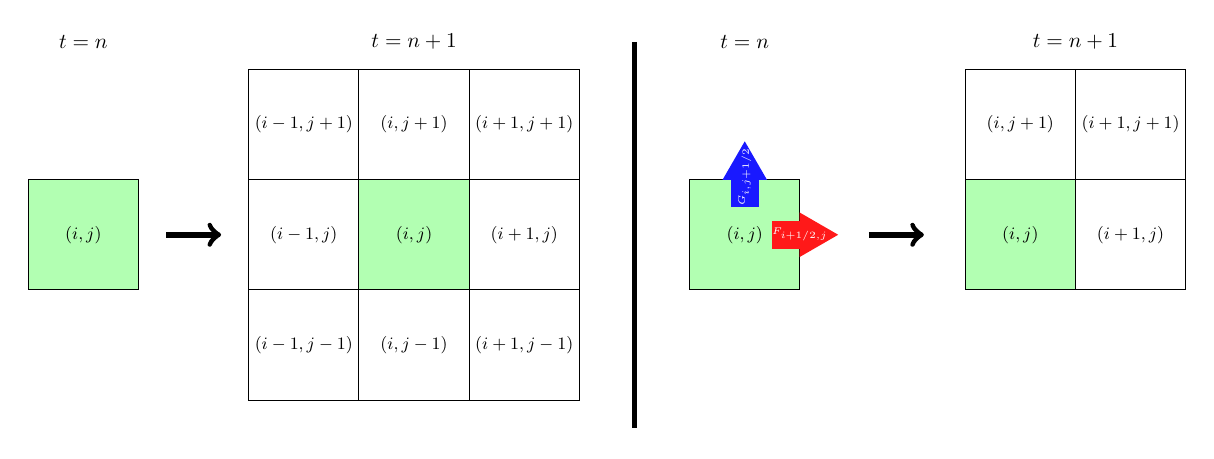
\begin{tikzpicture}[scale=0.7, transform shape]

   % Draw the center cell
    \filldraw[fill=green!30] (0,0) rectangle ++(2,2);
    
    % Draw the grid
    \foreach \i in {-2,0,2}
      \foreach \j in {-2,0,2} {
        \draw (\i,\j) rectangle ++(2,2);
      }

    % Draw a small square on the left with an arrow
    \filldraw[fill=green!30] (-6,0) rectangle ++(2,2);
    \draw[->, line width=2pt] (-3.5,1) -- (-2.5,1);

    % Coordinate points
    \node[font=\fontsize{9}{12}\selectfont] at (-5, 1) {$(i, j)$};
    \node[font=\fontsize{9}{12}\selectfont] at (1, 1) {$(i, j)$};
    \node[font=\fontsize{9}{12}\selectfont] at (3, 1) {$(i+1, j)$};
    \node[font=\fontsize{9}{12}\selectfont] at (-1, 1) {$(i-1, j)$};
    \node[font=\fontsize{9}{12}\selectfont] at (1, 3) {$(i, j+1)$};
    \node[font=\fontsize{9}{12}\selectfont] at (3, 3) {$(i+1, j+1)$};
    \node[font=\fontsize{9}{12}\selectfont] at (-1, 3) {$(i-1, j+1)$};
    \node[font=\fontsize{9}{12}\selectfont] at (1, -1) {$(i, j-1)$};
    \node[font=\fontsize{9}{12}\selectfont] at (3, -1) {$(i+1, j-1)$};
    \node[font=\fontsize{9}{12}\selectfont] at (-1, -1) {$(i-1, j-1)$};

    % Time steps
    \node[font=\fontsize{11}{12}\selectfont] at (-5, 4.5) {$t=n$};
    \node[font=\fontsize{11}{12}\selectfont] at (1, 4.5) {$t=n+1$};

    % Dividing line
    \draw[-, line width=2pt] (5,4.5) -- (5,-2.5);
    
     % Draw a small square on the left with an arrow
    \filldraw[fill=green!30] (6,0) rectangle ++(2,2);
    \draw[->, line width=2pt] (9.25,1) -- (10.25,1);

    \filldraw[fill=green!30] (11,0) rectangle ++(2,2);
    \draw (13,0) rectangle ++(2,2);
    \draw (11,2) rectangle ++(2,2);
    \draw (13,2) rectangle ++(2,2);

    % Coordinate points
    \node[font=\fontsize{9}{12}\selectfont] at (7, 1) {$(i, j)$};
    \node[font=\fontsize{9}{12}\selectfont] at (12, 1) {$(i, j)$};
    \node[font=\fontsize{9}{12}\selectfont] at (14, 1) {$(i+1, j)$};
    \node[font=\fontsize{9}{12}\selectfont] at (12, 3) {$(i, j+1)$};
    \node[font=\fontsize{9}{12}\selectfont] at (14, 3) {$(i+1, j+1)$};

    % Time steps
    \node[font=\fontsize{11}{12}\selectfont] at (7, 4.5) {$t=n$};
    \node[font=\fontsize{11}{12}\selectfont] at (13, 4.5) {$t=n+1$};

    \filldraw[fill=blue!90,draw=none] (6.75,1.5) rectangle ++(0.5,0.5);
    \filldraw[fill=red!90,draw=none] (7.5,0.75) rectangle ++(0.5,0.5);

    \node[isosceles triangle, isosceles triangle apex angle=60, draw=none, rotate=90, fill=blue!90, minimum size =0.7cm] (T90)at (7,2.2){};

    \node[isosceles triangle, isosceles triangle apex angle=60, draw=none, fill=red!90, minimum size =0.7cm] (T90)at (8.2,1){};

    \node[font=\fontsize{5}{8}\selectfont,color=white] at (8, 1) {$F_{i+1/2, j}$};
    \node[font=\fontsize{5}{8}\selectfont,color=white, rotate=90] at (7, 2.05) {$G_{i, j+1/2}$};
    
    
  \end{tikzpicture}
  \caption{Two-dimensional schematic demonstrating the difference in the creation procedure of the ({\it left}) legacy implementation vs. the ({\it right}) current implementation. The {\it green} cell represents one with a probability above the threshold, and the downwind fluxes $F_{i+1/2,j}$ and $G_{i,j+1/2}$ represent the probability flow at the half-step forward $x$- and $y$-interfaces, respectively.}
  \label{fig:Creation}
\end{figure}

\paragraph{Deletion of cells.} 

For the deletion process, the legacy implementation checks all directions to ensure that a considered cell neighbors no cells with probability above threshold before deleting it from the tree. Checking every neighbor is a redundancy that results in saving useless cells, as only the \textit{upwind} cells can advect probability into the cell of interest. Therefore, the current implementation cuts down on the number of cells checked along the entire grid for each time step, as is demonstrated schematically in Figure~\ref{fig:Deletion}. 

\begin{figure}[htb]
  \centering
  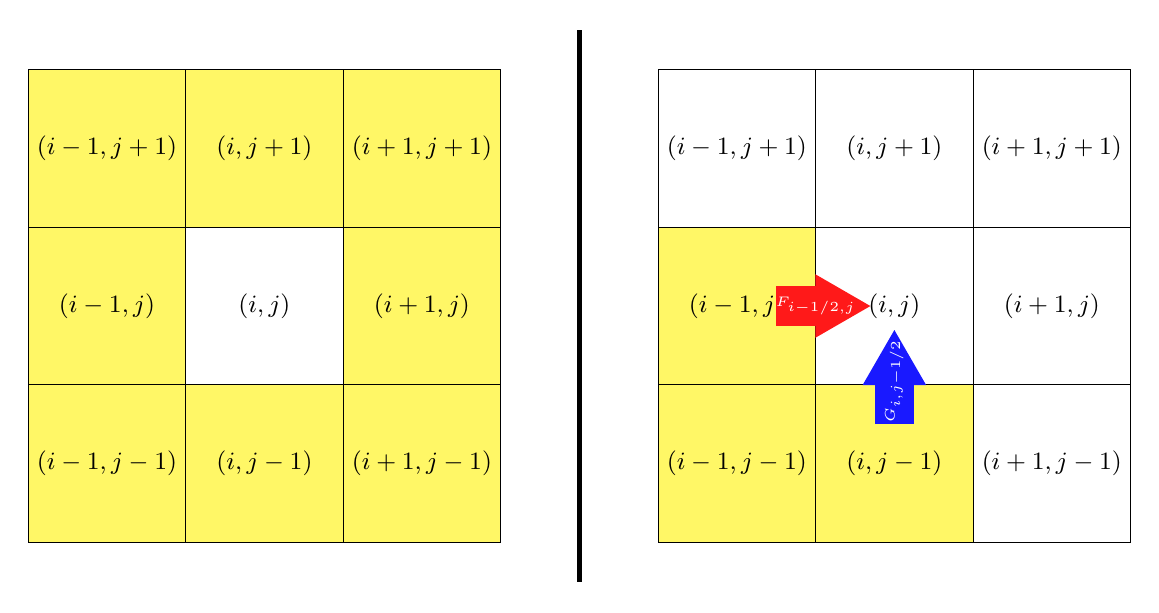
\begin{tikzpicture}[scale=1, transform shape]
    
    % Draw the grid
    \foreach \i in {-2,0,2}
      \foreach \j in {-2,0,2} {
        \filldraw[fill=yellow!60] (\i,\j) rectangle ++(2,2);
      }

       % Draw the center cell
    \filldraw[fill=white!60] (0,0) rectangle ++(2,2);


    % Coordinate points
    \node[font=\fontsize{9}{12}\selectfont] at (1, 1) {$(i, j)$};
    \node[font=\fontsize{9}{12}\selectfont] at (3, 1) {$(i+1, j)$};
    \node[font=\fontsize{9}{12}\selectfont] at (-1, 1) {$(i-1, j)$};
    \node[font=\fontsize{9}{12}\selectfont] at (1, 3) {$(i, j+1)$};
    \node[font=\fontsize{9}{12}\selectfont] at (3, 3) {$(i+1, j+1)$};
    \node[font=\fontsize{9}{12}\selectfont] at (-1, 3) {$(i-1, j+1)$};
    \node[font=\fontsize{9}{12}\selectfont] at (1, -1) {$(i, j-1)$};
    \node[font=\fontsize{9}{12}\selectfont] at (3, -1) {$(i+1, j-1)$};
    \node[font=\fontsize{9}{12}\selectfont] at (-1, -1) {$(i-1, j-1)$};

    % Dividing line
    \draw[-, line width=2pt] (5,4.5) -- (5,-2.5);

     % Draw the grid
     \foreach \i in {6,8,10}
      \foreach \j in {-2,0,2} {
        \filldraw[fill=white!60] (\i,\j) rectangle ++(2,2);
      }
    \foreach \i in {6,8}
      \foreach \j in {-2,0} {
        \filldraw[fill=yellow!60] (\i,\j) rectangle ++(2,2);
      }

       % Draw the center cell
    \filldraw[fill=white!60] (8,0) rectangle ++(2,2);

    % Coordinate points
    \node[font=\fontsize{9}{12}\selectfont] at (9, 1) {$(i, j)$};
    \node[font=\fontsize{9}{12}\selectfont] at (11, 1) {$(i+1, j)$};
    \node[font=\fontsize{9}{12}\selectfont] at (7, 1) {$(i-1, j)$};
    \node[font=\fontsize{9}{12}\selectfont] at (9, 3) {$(i, j+1)$};
    \node[font=\fontsize{9}{12}\selectfont] at (11, 3) {$(i+1, j+1)$};
    \node[font=\fontsize{9}{12}\selectfont] at (7, 3) {$(i-1, j+1)$};
    \node[font=\fontsize{9}{12}\selectfont] at (9, -1) {$(i, j-1)$};
    \node[font=\fontsize{9}{12}\selectfont] at (11, -1) {$(i+1, j-1)$};
    \node[font=\fontsize{9}{12}\selectfont] at (7, -1) {$(i-1, j-1)$};

    \filldraw[fill=blue!90,draw=none] (8.75,-0.5) rectangle ++(0.5,0.5);
    \filldraw[fill=red!90,draw=none] (7.5,0.75) rectangle ++(0.5,0.5);

    \node[isosceles triangle, isosceles triangle apex angle=60, draw=none, rotate=90, fill=blue!90, minimum size =0.7cm] (T90)at (9,0.2){};

    \node[isosceles triangle, isosceles triangle apex angle=60, draw=none, fill=red!90, minimum size =0.7cm] (T90)at (8.2,1){};

    \node[font=\fontsize{5}{8}\selectfont,color=white] at (8, 1) {$F_{i-1/2, j}$};
    \node[font=\fontsize{5}{8}\selectfont,color=white, rotate=90] at (9, 0.05) {$G_{i, j-1/2}$};

  \end{tikzpicture}
  \caption{Two-dimensional schematic demonstrating the difference in the deletion procedure of the ({\it left}) legacy implementation vs. the ({\it right}) current implementation. The {\it white} cell represents one with a probability below the threshold, and the {\it yellow} cells are the neighbors checked for probability above the threshold value by the algorithm. The upwind fluxes $F_{i-1/2,j}$ and $G_{i,j-1/2}$ represent the probability flow at the half-step back $x$- and $y$-interfaces, respectively.}
  \label{fig:Deletion}
\end{figure}

Additionally, the current algorithm considers the frequency of the deletion procedure. The purpose of pruning low-probability cells from the BST is to decrease the total number of Riemann problems that need to be solved at each grid cell interface. However, the deletion procedure requires an exhaustive search of the entire BST, and in certain cases, the time saved on time-marching fewer cells is not worth the process of deletion. Therefore, the current implementation makes the deletion frequency a parameter, and tunes it empirically. 

\subsection{Time-step adaptivity}

Stability is an important consideration when designing numerical methods. To ensure stability when time-marching discretized functions through phase space, the size of the time step must adhere to the magnitude of the rate of change, so information does not ``skip'' grid cells, which would cause the scheme to accumulate errors. The Courant–Friedrichs–Lewy (CFL) convergence condition \cite{CFL} ensures stability for time-integration schemes by defining the time step $\Delta t$ as a function of $C_{\max}$:
\begin{equation}\label{eq:CFL}
    \Delta t \leq \min \Bigg[ C_{\max} \Bigg(\sum_{i=1}^n \frac{f_i(\mathbf{x})}{\Delta x_i} \Bigg)^{-1} \quad \forall\, \mathbf{x} \in \Omega \Bigg],
\end{equation}
where $C_{\max}=1$ for explicit time schemes, and $\Omega$ represents the entire domain of phase space where $p_{\mathbf{x}}(\mathbf{x}',t) \geq \bar{p}$. When propagating a numerical scheme governed by chaotic dynamics, there are quiescent, slow-changing periods ($|\mathbf{f}(\mathbf{x})|$ is small) and there are chaotic, fast-changing periods ($|\mathbf{f}(\mathbf{x})|$ is large). Fixed time-step schemes must adhere to the most chaotic period of the entire trajectory, even through the more stable quiescent periods, where larger time steps could achieve stability. The legacy implementation of GBEES uses this inefficient, fixed time-step method tuned empirically to ensure stability of the scheme, a subprocedure that is also computationally wasteful. Therefore, to address these numerical limitations, we utilize an adaptive time-step approach, where $\Delta t$ is determined via Eq.~\eqref{eq:CFL} at each step. 

\subsection{Current vs. legacy implementation}
Altogether, the changes proposed to the legacy implementation of GBEES improve the overall time complexity of the algorithm, speeding up the process of propagating a three-dimensional PDF in the Lorenz attractor system as demonstrated by Figure~\ref{fig:Comparison}. Note that although the number of cells required to describe the PDF is lower for the current implementation due to the creation and deletion improvements, the overall shape of growth is the same. However, the shapes of the program run-time are different, demonstrating that the current implementation has an improved time complexity compared to the legacy counterpart. This efficiency improvement allows the algorithm to feasibly be applied to higher-dimensional problems, specifically propagating orbital uncertainty for nonlinear, chaotic systems. 

\begin{figure}[htb]
	\centering\includegraphics[width=0.95\textwidth, trim=2.5cm 0 0.9cm 0]{Figures/Lorenz3D/Timing.eps}
	\caption{Comparison of legacy implementation with the current implementation of GBEES. This comparison was performed on the 3D Lorenz attractor from Figure~\ref{fig:3DLorenz}.}
	\label{fig:Comparison}
\end{figure}

\section{Planar, circular, restricted three-body problem}

The restricted three-body problem considers the motion of an object with negligible mass in a system of two massive bodies that orbit about their respective center of mass, unaffected by the object of negligible mass. Assuming the orbit of the two massive bodies about the center of mass is circular, and the motion of the object is constrained to the plane of orbit, the result is the planar, circular, restricted three-body problem \cite{jG97} (PCR3BP). In the barycentric, dimensionless, rotating coordinate frame, the equations of motion of the object are
\begin{gather}\label{eq:PCR3BP_2nd}
    \notag \ddot{x}-2\,\dot{y} = \Omega_x,\\ 
    \ddot{y}+2\,\dot{x} = \Omega_y,\\ \notag  
    \textrm{where} \quad \Omega(x,y) = \frac{x^2+y^2}{2}+\frac{1-\mu}{r_1}+\frac{\mu}{r_2}+\frac{\mu(1-\mu)}{2},
\end{gather}
$\mu$ is the gravitational parameter of the two-body system, $r_1$ is the distance to the primary body, and $r_2$ is the distance to the secondary body. 

In the PCR3BP, there exist five equilibrium points $L_1$--$L_5$, known as Lagrange or libration points \cite{sR22}, that lie in the plane of orbit and are at rest in the synodic frame. $L_1$, $L_2$, and $L_3$ are collinear, while $L_4$ and $L_5$ form equilateral triangles with the two massive bodies. 
\begin{figure}[htb]
\centering
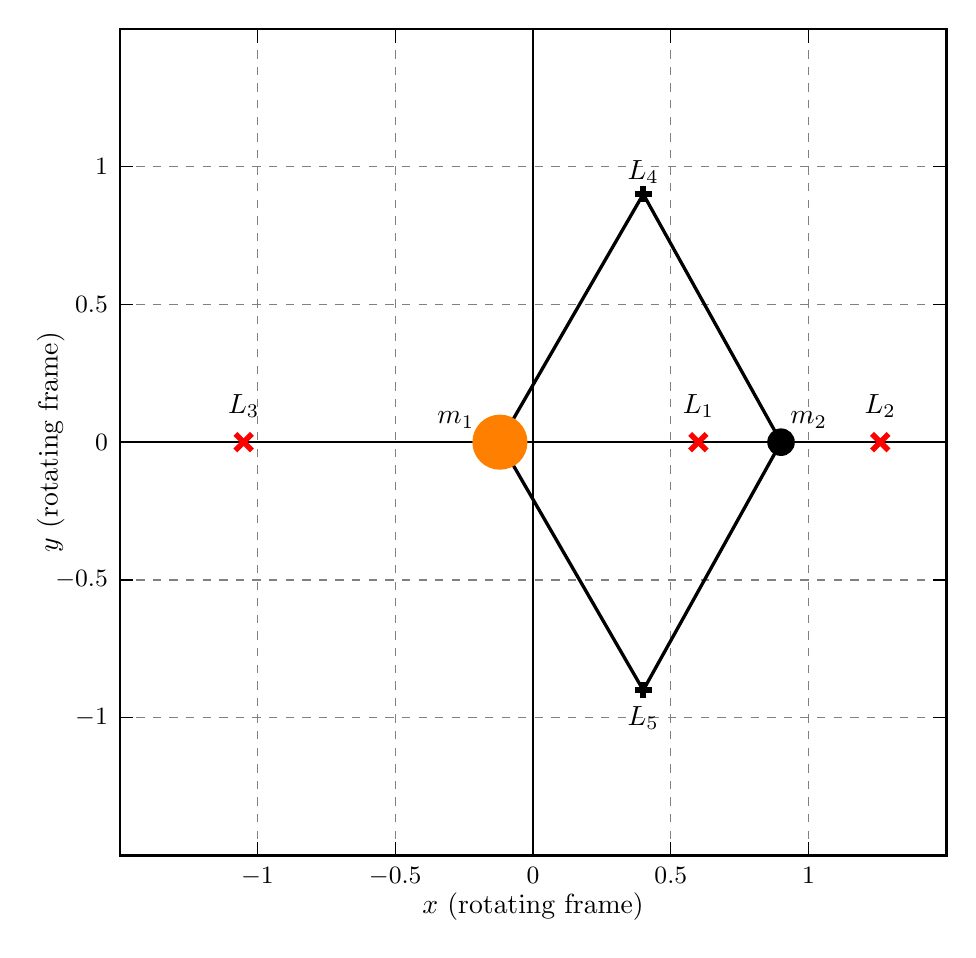
\begin{tikzpicture}[scale=3.5]

% Draw the grid
\draw[gray, dashed] (-1.5,-1.5) grid[step=0.5] (1.5,1.5);

% Draw the axes
\draw[thick,-] (-1.5,0) -- (1.5,0);
\draw[thick,-] (0,-1.5) -- (0,1.5);

% Draw x ticks and labels
\foreach \x/\label in {-1/{-1}, -0.5/{-0.5}, 0/{0}, 0.5/{0.5}, 1/{1}}
{
    \draw (\x,-1.5) -- (\x,-1.45) node[below, font = \fontsize{9}{12}\selectfont, yshift=-2mm] {$\label$};
}

\foreach \x/\label in {-1/{-1}, -0.5/{-0.5}, 0/{0}, 0.5/{0.5}, 1/{1}}
{
    \draw (\x,1.5) -- (\x,1.45);
}

% Draw y ticks
\foreach \y/\label in {-1/{-1}, -0.5/{-0.5}, 0/{0}, 0.5/{0.5}, 1/{1}}
{
    \draw (-1.5,\y) -- (-1.45,\y) node[left, font = \fontsize{9}{12}\selectfont, xshift=-2mm] {$\label$};
}

\foreach \y/\label in {-1/{-1}, -0.5/{-0.5}, 0/{0}, 0.5/{0.5}, 1/{1}}
{
    \draw (1.5,\y) -- (1.45,\y);
}

% Set axis limits
\draw[thick] (-1.5,0) -- (1.5,0);
\draw[thick] (0,-1.5) -- (0,1.5);

% Draw the square outline
\draw[thick] (-1.5,-1.5) rectangle (1.5,1.5);

% Add x label
\node[below] at (0,-1.6) {$x$ (rotating frame)};

% Add y label
\node[rotate=90] at (-1.75,0) {$y$ (rotating frame)};

\draw[black, line width=1.2pt] (-0.12,0) -- (0.4,0.9);
\draw[black, line width=1.2pt] (-0.12,0) -- (0.4,-0.9);
\draw[black, line width=1.2pt] (0.9,0) -- (0.4,0.9);
\draw[black, line width=1.2pt] (0.9,0) -- (0.4,-0.9);

% Add orange filled circle labeled m_1 
\fill[orange] (-0.12,0) circle (0.1);
\node[black] at (-0.28,0.08) {$m_1$};

% Add orange filled circle labeled m_1 
\fill[black] (0.9,0) circle (0.05);
\node[black] at (1,0.08) {$m_2$};

% L1
\draw[red, line width=2pt] (0.57,-0.03) -- (0.63,0.03);
\draw[red, line width=2pt] (0.57,0.03) -- (0.63,-0.03);
\node[black] at (0.6,0.13) {$L_1$};

% L2
\draw[red, line width=2pt] (1.23,-0.03) -- (1.29,0.03);
\draw[red, line width=2pt] (1.23,0.03) -- (1.29,-0.03);
\node[black] at (1.26,0.13) {$L_2$};

% L3
\draw[red, line width=2pt] (-1.02,-0.03) -- (-1.08,0.03);
\draw[red, line width=2pt] (-1.02,0.03) -- (-1.08,-0.03);
\node[black] at (-1.05,0.13) {$L_3$};

% L4
\draw[black, line width=2pt] (0.37,0.9) -- (0.43,0.9);
\draw[black, line width=2pt] (0.4,0.93) -- (0.4,0.87);
\node[black] at (0.4,0.98) {$L_4$};

% L5
\draw[black, line width=2pt] (0.37,-0.9) -- (0.43,-0.9);
\draw[black, line width=2pt] (0.4,-0.93) -- (0.4,-0.87);
\node[black] at (0.4,-1) {$L_5$};

\end{tikzpicture}
\caption{Schematic of the Lagrange points in the synodic, dimensionless coordinate frame.}
	\label{fig:Libration_points}
\end{figure}

In the vicinity of these equilibrium points, there exist initial conditions that result in quasi-periodic orbits (QPOs) about the libration points. Multiple spacecraft have operated in these orbits \cite{ISEE-3, SOHO} as they require minimal propulsion to maintain. The class of quasi-periodic orbits that lie entirely in the plane of the two massive bodies are known as Lyapunov orbits\cite{vS67}. Extensive research has been conducted to accurately calculate the initial conditions of these orbits\cite{rF73}, to such an extent that precomputed catalogs, like the {\it JPL Three-Body Periodic Orbit Catalog}\cite{JPL3BO}, store the initial conditions for QPOs about all three collinear libration points for various planetary systems. As the initial conditions for these periodic orbits are readily available, and the orbits themselves are low-fidelity representations of true spacecraft motion, we view this as a prudent starting point for the application of GBEES to higher dimensions.

To govern the advection term of Eq.~\eqref{eq:FPE} by the equations of motion of the PCR3BP, Eq.~\eqref{eq:PCR3BP_1st} must be converted from a $2^{\textrm{nd}}$-order ODE to a $1^{\textrm{st}}$-order ODE. In $1^{\textrm{st}}$-order form, the state $\mathbf{x}$ and the equations of motion $d\mathbf{x}/dt$ of the PCR3BP become
\begin{equation}\label{eq:PCR3BP_1st}
    \mathbf{x} = \begin{bmatrix}x\\y\\v_x\\v_y\end{bmatrix}, \quad \frac{d\mathbf{x}}{dt} = \mathbf{f}(\mathbf{x}) = \begin{bmatrix}
v_x \\[0.25em] v_y \\[0.25em] 2v_y + x - \frac{\mu(x-1+\mu)}{\Big((x-1+\mu)^2+y^2\Big)^{3/2}}-\frac{(1-\mu)(x+\mu)}{\Big((x+\mu)^2+y^2\Big)^{3/2}} \\[0.25em] -2v_x + y - \frac{\mu y}{\Big((x-1+\mu)^2+y^2\Big)^{3/2}}-\frac{(1-\mu) y}{\Big((x+\mu)^2+y^2\Big)^{3/2}}
\end{bmatrix}.
\end{equation}
The result is a four-dimensional nonlinear system, a useful and relevant test case with increased complexity for the new and improved GBEES algorithm. To visualize the 4D PDFs generated and propagated, we create two 2D PDFs by integrating $p_{\mathbf{x}}(\mathbf{x}',t)$ over the velocity space for the position PDF $p_{(x,y)}(x',y',t)$, and by integrating $p_{\mathbf{x}}(\mathbf{x}',t)$ over the position space for the velocity PDF $p_{(v_x,v_y)}(v_x',v_y',t)$:
\begin{subequations}
\begin{gather}
    p_{(x,y)}(x',y',t) = \int_{\Omega_{(v_x,v_y)}} p_{\mathbf{x}}(\mathbf{x}',t)dv_x'dv_y', \\ 
    \quad p_{(v_x,v_y)}(v_x',v_y',t) = \int_{\Omega_{(x,y)}} p_{\mathbf{x}}(\mathbf{x}',t)dx'dy',
\end{gather}
\end{subequations}
where $\Omega_{(x,v)}$ and $\Omega_{(v_x,v_y)}$ represent the entire domain of the PDF over position and velocity, respectively. Utilizing the initial conditions precomputed in the JPL Three-Body Periodic Orbit catalog, we possess a complete framework for propagating a four-dimensional PDF representing the uncertainty of an object in a Lyapunov orbit. We now demonstrate the flexibility of this extension of GBEES given various physical scenarios where we speculate the EKF may perform poorly. 

\section{Infrequently observed Jupiter-Europa trajectory}

As space missions venture further into the depths of the Solar System, novel methods for guidance and navigation become imperative due to the limitations of the legacy standard, wherein commands are uplinked based on downlinked measurements received prior, communicated via the Deep Space Network (DSN). One such limitation is that, at such extreme distances from Earth, data communication between spacecraft and ground control has significant light time delays (i.e., approximately an hour and a half at Jupiter) that complicate navigation in environments where uncertain dynamics require trajectory control on timescales under the light time delay (i.e., repeated low altitude flybys of a Jovian or Saturnian moon). Second, a non-autonomous approach requires a reserved DSN antenna for uplink and downlink, which may not always be feasible as the number of deep-space missions grows \cite{sB17,sB19}. NASA's Deep Space 1\cite{sB98,jR00} (DS1) avoided these limitations by employing an autonomous navigation system, AutoNav, that utilized on-board imagery of nearby asteroids to autonomously determine its trajectory in space and compute necessary maneuvers (a.k.a. OpNav). One drawback of utilizing OpNav using main belt asteroids is that cataloged asteroids beyond the main belt are fewer and far between, making measurements updates less frequent (DS1 planned to utilize AutoNav at roughly weekly intervals\cite{sB12}). In chaotic regimes, this will result in the uncertainty of a spacecraft spreading widely over phase space. To maintain custody of spacecraft operating in QPOs in these regimes using autonomous navigation, operational orbits must be relatively stable such that infrequent measurements will not result in accidental reentry or escape. 

Given the physical scenario described, the nominal trajectory chosen for uncertainty propagation will be relatively stable and discrete measurement updates will be infrequent. The EKF assumes that the errors in estimation due to the utilization of a linearized propagation model are corrected via frequent measurement updates \cite{pG12}. However, in the trajectory we have outlined, measurement updates partially rely upon the presence of nearby cataloged asteroids, thereby diminishing our confidence in the assumption of frequency. Conversely, conducting uncertainty propagation via a MC simulation requires an unknown-but-substantial number of particles to ensure a sufficient level of confidence in the approximated distribution. Without knowledge of the posterior distribution prior to the following measurement update, defining what qualifies as ``substantial'' may be fairly unpredictable. For normal distributions, there are formulae following from the Central Limit Theorem that provide the number of particles required to achieve some confidence level of the final, approximated distribution \cite{wO15}. However, for non-Gaussian distributions, determining this optimal number is less straightforward \cite{vE16}. This often leads to an excessive number of initialized particles, ultimately squandering computational resources. 

We utilize a set of initial conditions that result in a Lyapunov orbit about the $L_3$ Jupiter-Europa libration point, sourced from the JPL Three-Body Periodic Orbit catalog (initial conditions can be found in Table~\ref{tab:Jupiter-Europa} and are relative to the Jupiter-Europa barycenter). We assume an initial uncertainty in position of $10^3$ km and velocity of $10^{-1}$ km/s, as is the assumed \textit{a priori} uncertainty for spacecraft near Jupiter utilizing autonomous navigation \cite{nS08}. To test both the accuracy and efficiency of GBEES, we initialize a MC simulation with the same initial conditions and uncertainty. We propagate the uncertainty using both GBEES and the MC simulation through one full period of the Lyapunov orbit ($\sim 3.5$ days), with a discrete measurement update every 
1/3 of the orbit ($\sim 1.17$ days). Measurements are assumed to be the state of the nominal trajectory at the given epoch, with uncertainty in position and velocity of the measurement being equal to the initial uncertainty.

\begin{table}[htbp]
    \caption{Initial conditions of a $L_3$ Jupiter-Europa Lyapunov trajectory.}
   \label{tab:Jupiter-Europa}
    \centering
   \begin{tabular}{| c | c | c | c |} % Column formatting, 
      \hline 
     $x_0\pm \Delta x_0$ (km)  & $y_0\pm \Delta y_0$ (km) & ${v_x}_0 \pm \Delta {v_x}_0$ (km/s) & ${v_y}_0 \pm \Delta {v_y}_0$ (km/s)\\
      \hline 
      $(-9.55341 \pm 0.01)$\num{e5} &  $(0.00 \pm 0.01)$\num{e5} &  $(0.00 \pm 0.01)$\num{e1}	& $(1.09711 \pm 0.01)$\num{e1}	\\
      \hline
   \end{tabular}
\end{table}

\begin{figure}[h]
    \centering\includegraphics[width=0.45\textwidth, trim=1.2cm 0 0.5cm 0]{Figures/Jupiter-Europa/Position.eps} 
    \centering\includegraphics[width=0.45\textwidth, trim=1.2cm 0 0.5cm 0]{Figures/Jupiter-Europa/Velocity.eps}
    \centering\includegraphics[width=0.45\textwidth, trim=1.2cm 0 0.5cm 0]{Figures/Jupiter-Europa/Position_MC.eps}
    \centering\includegraphics[width=0.45\textwidth, trim=1.2cm 0 0.5cm 0]{Figures/Jupiter-Europa/Velocity_MC.eps}
    \caption{Initially Gaussian uncertainty time-marched with GBEES governed by the PCR3BP in the Jupiter-Europa system. ({\it top}) The contour plots represent the PDF propagated by GBEES about the nominal trajectory. $M_1$, $M_2$, and $M_3$ denote the epochs where discrete measurement updates take place, with $M_1$ being the initialization of the simulation. Note that the {\it colors} of the contours representing the magnitude of the probability of a PDF are not relative to other PDFs, but instead are representative of probability differences throughout the individual distributions. ({\it bottom}) GBEES compared with a 500 particle MC simulation, to confirm the accuracy of the method. A complete list of the simulation parameters can be found in Table~\ref{tab:GBEES_parameters}.}
    \label{fig:JE_results}
\end{figure}

Figure~\ref{fig:JE_results} depicts the results of the described $L_3$ Jupiter-Europa Lyapunov trajectory simulation. The initially Gaussian uncertainty beginning from the $M_1$ epoch rapidly spreads over phase space (the uncertainty in $y$ goes from being on the order of $10^3$ km to $10^5$ km after only about $1.17$ days). Via comparison with the MC simulation, we validate that GBEES has accurately propagated the uncertainty between measurement updates. Figure~\ref{fig:JE_timing} provides the computational efficiency comparison of a RK4 time-marching MC simulation with GBEES over the trajectory of interest. To ensure the MC simulation provides the same ``quantity of information'' at each measurement epoch $M_i$ for $i=1,2,3$, we set the number of particles in the MC simulation equal to number of cells with probability above threshold in the final PDF at $M_i$ for $i=1,2,3$. Unlike GBEES, which propagates a discretized grid that grows in size with the uncertainty, MC simulations have no mechanism for refining the distribution it is propagating as it spreads over phase space. Therefore, the MC simulation has the disadvantage of having to time-march a large quantity of particles even when the uncertainty is relatively small so that it may represent the uncertainty when it is relatively large. The discrete changes in the number of cells for both methods in Figure~\ref{fig:JE_timing} is representative of discrete Bayesian updates in the case of GBEES and resamplings from the new measurements in the case of the MC simulation. This is another important consideration when comparing the results of the two simulation methods; GBEES uses Bayes' theorem to update based on a discrete measurement, which considers both the \textit{a priori} distribution as well as the measurement update. Conversely, the MC simulation disregards the prior distribution completely and resamples based on the new measurement update. We consider this to be a potential cause for the slight divergence of the final distributions of GBEES and the MC simulation at each $M_i$ in Figure~\ref{fig:JE_results}. 

\begin{figure}[t]
    \centering\includegraphics[width=0.8\textwidth, trim=2.2cm 0 1.6cm 0]{Figures/Jupiter-Europa/Timing.eps}
    \caption{Comparing the computational time of GBEES vs. MC when propagating uncertainty for the trajectory from Figure~\ref{fig:JE_results}. Discrete jumps in the number of cells tracked by each uncertainty propagation method are representative of discrete Bayesian updates in GBEES's case and resamplings in the MC simulation's case.}
    \label{fig:JE_timing}
\end{figure}

\begin{comment}
\section{Unstable, frequently observed Earth-Moon trajectory}

The growth of the number of defunct and derelict pieces of human-made spacecraft, known as space debris, in low-Earth orbit (LEO) is a looming concern for space sustainability. Along with active debris removal (ADR) technologies, LEO space debris catalogs and models \cite{LEOLabs, ORDEM3} are regularly updated for the purpose of conjunction analysis and, more broadly, to mitigate the likelihood of the infamous Kessler Syndrome. Contrarily, xGEO to cislunar space, which encompasses the region from GEO to the Moon's orbit, is significantly less regulated and maintained (although recent work has been done to establish these catalogs\cite{rF21}). While risk of collision with debris in cislunar space is currently low due to the small number of objects orbiting in the regime's vastness, this will likely change soon; as space programs across the globe push to establish consistent lunar presences, the number of objects in this regime, as well as the risk of collision, will increase. Additionally, due to the increased distance from Earth compared with LEO space debris, optical and radar detections of cislunar debris will have higher associated uncertainties, meaning less predictability in regards to conjunction analysis and collision avoidance. 

Ensuring the continued safety of spacecraft operating in the xGEO to cislunar regime requires novel uncertainty propagation methods, like the one proposed, applied to derelict space debris. We demonstrate GBEES on a piece of space debris in a Lyapunov orbit about the $L_1$ Earth-Moon libration point. $L_1$ and $L_2$ Lyapunov orbits in general are relatively unstable due to their being saddle equilibrium points, thus the state uncertainty spreads quickly. Due to this instability, frequent measurements are required to confirm that collision with any neighboring spacecraft is unlikely. In these scenarios, MC simulations tend to be computationally expensive, as each new observation requires a complete resampling from the new measurement distribution. Additionally, when a new measurement is obtained, all prior information from the MC simulation is disregarded, which can be a problem when measurements are inaccurate. Conversely, GBEES easily handles discrete measurement updates via Eq.~\eqref{eq:Bayes}, considering both the distribution prior to the measurement as well as the measurement itself. 

We utilize a set of initial conditions that result in a Lyapunov orbit about the $L_1$ Earth-Moon point, sourced from the JPL Three-Body Periodic Orbit catalog (initial conditions can be found in Table~\ref{tab:Earth-Moon} and are relative to the Earth-Moon barycenter). We assume an initial uncertainty in position of $10$ km and velocity of $10^{-3}$ km/s, as is standard for optical measurements of objects in the cislunar regime \cite{cC22, jB22}. To test both the accuracy and efficiency of GBEES, we initialize a MC simulation with the same initial conditions and uncertainty. We propagate the uncertainty using both GBEES and the MC simulation through one full period of the Lyapunov orbit ($\sim 29$ days), with a discrete measurement update every 1/60 of the orbit ($\sim 0.5$ days). Measurements are assumed to be the state of the nominal trajectory at the given epoch, with uncertainty in position and velocity of the measurement being equal to the initial uncertainty. 

\begin{table}[htbp]
    \caption{Initial Conditions of $L_1$ Earth-Moon Lyapunov Trajectory}
   \label{tab:Earth-Moon}
    \centering
   \begin{tabular}{| c | c | c | c |} % Column formatting, 
      \hline 
     $x_0\pm \Delta x_0$ (km)  & $y_0\pm \Delta y_0$ (km) & ${v_x}_0 \pm \Delta {v_x}_0$ (km/s) & ${v_y}_0 \pm \Delta {v_y}_0$ (km/s)\\
      \hline 
       $(2.52157 \pm 0.0001)$E5& $(0.0 \pm 0.0001)$E5  &  $(0.0 \pm 0.01)$E-1	& $(7.72379 \pm 0.01)$E-1	\\
      \hline
   \end{tabular}
\end{table}
\end{comment}

\section{Consideration of epistemic uncertainty for solar probes}

Of the limitations of existing uncertainty propagation methods, the most concerning for space missions delving into unexplored domains may be their failure to consider epistemic uncertainty. Epistemic uncertainty, or uncertainty of the model, may be negligible in regimes where perturbations from solar radiation pressure, atmospheric drag, zonal harmonics, etc., are either well-defined or relatively small. However, this may not be true for all realms of space. Consider the Parker Solar Probe\cite{Parker}, a NASA spacecraft designated with the task of flying through the Sun's upper atmosphere to take measurements and expand our understanding of solar wind. In this unexplored regime (the Parker Solar probe flies seven times closer to the Sun than any spacecraft has ever flown), the effect of solar radiation pressure on the motion of the spacecraft is not well-defined, thus the model representing the motion of the probe has some non-negligible, associated uncertainty. To account for this, Eq.~\eqref{eq:FPE} includes the diffusion term (i.e. $Q \neq 0$) which is representative of random motion. In 2D (with higher-dimensional cases following as obvious extensions), the diffusion term is added to Eq.~\eqref{eq:FPE_discretized} by updating the fluxes such that, for all $(i,j)$,
\begin{subequations}
\begin{gather}\label{eq:diffusion_correction}
F^n_{i+1/2,j} += \bar{\mu}_x\frac{\Delta p^n_{i+1/2,j}}{\Delta x}, \\
G^n_{i,j+1/2} += \bar{\mu}_y\frac{\Delta p^n_{i,j+1/2}}{\Delta y},
\end{gather}
\end{subequations}
where $\bar{\boldsymbol{\mu}} = [\bar{\mu}_x \,\,\, \bar{\mu}_y]$ is the coefficient of diffusion and can be tuned depending on how uncertain the model definition is. %An important consideration when including diffusion in GBEES is that the creation and deletion procedures revert back to their legacy implementations, as diffusion may cause probability to flow upwind depending upon the relative differences between cells. 

We choose a set of initial conditions that result in a Lyapunov orbit about the $L_3$ libration point of the Sun-Earth system, (initial conditions can be found in Table~\ref{tab:Sun-Earth} and are relative to the Sun-Earth barycenter). This specific set of initial conditions takes the spacecraft to a distance of nearly 7 million km from the Sun at perihelion (the Parker Solar Space probe's closest approach is 6.16 million km from the Sun). Considering epistemic uncertainty is non-negligibile, we include the diffusion term in the numerical solution of Eq.~\eqref{eq:FPE} and set $\bar{\boldsymbol{\mu}} = [1\num{e-5} \,\,\, 1\num{e-5} \,\,\, 1\num{e-5} \,\,\, 1\num{e-5}]$ (this choice of diffusion coefficient is proportional to the grid width and was tuned empirically). To test the limitations of GBEES, we assume an unrealistic, worst-case scenario initial uncertainty in position of $10^4$ km and velocity of 1 km/s. This measurement uncertainty is much larger than is estimated for the Parker Solar Probe \textit{a priori} uncertainties \cite{dJ17}. We initialize a MC simulation with the same initial conditions and uncertainty. From the entire orbit of the chosen initial conditions, we propagate uncertainty through a portion of the close approach, as this section of the orbit will be most affected by epistemic uncertainty. No discrete measurement updates are taken in this simulation.

\begin{table}[htbp]
    \caption{Initial conditions of a $L_3$ Sun-Earth Lyapunov trajectory.}
   \label{tab:Sun-Earth}
    \centering
    \resizebox{.99\hsize}{!}{$
   \begin{tabular}{| c | c | c | c | c |} % Column formatting, 
      \hline 
     & $x_0\pm \Delta x_0$ (km)  & $y_0\pm \Delta y_0$ (km) & ${v_x}_0 \pm \Delta {v_x}_0$ (km/s) & ${v_y}_0 \pm \Delta {v_y}_0$ (km/s)\\
      \hline 
      Full orbit & (-2.91781 $\pm$ 0.0001)\num{e8} & (0.0 $\pm$ 0.0001)\num{e8} &  (0 $\pm$ 100)\num{e-2} & (6.01321 $\pm$ 100)\num{e-2} \\
      \hline 
      Close approach & (-0.25536 $\pm$ 0.001)\num{e7} & (1.19445 $\pm$ 0.001)\num{e7} & (-8.98694 $\pm$ 0.1)\num{e1} & (-11.0549 $\pm$ 0.1)\num{e1} \\
      \hline
   \end{tabular}$}
\end{table}

\begin{figure}[htb]
    \centering\includegraphics[width=0.49\textwidth, trim=1.5cm 0 0.3cm 0]{Figures/Sun-Earth/Full_Orbit_Pos.eps}
    \centering\includegraphics[width=0.49\textwidth, trim=1.5cm 0 0.3cm 0]{Figures/Sun-Earth/Full_Orbit_Vel.eps}
    \caption{({\it left}) Position and ({\it right}) velocity in barycentric, synodic coordinate frame of $L_3$ Sun-Earth Lyapunov trajectory with initial conditions from Table~\ref{tab:Sun-Earth}. Period of full Lyapunov orbit is 365.2554 days, and total time of close approach trajectory is 1.8263 days.}
    \label{fig:SE_traj}
\end{figure}

Figure~\ref{fig:SE_results} provides the results of propagating the uncertainty of a solar probe through a close approach. To emphasize the effects of the inclusion of the diffusion term, we provide Figure~\ref{fig:SE_compare}, which compares the final position distributions of the Sun-Earth simulation excluding diffusion (i.e. $Q=0$) and including diffusion (i.e. $Q\neq0$). Figure~\ref{fig:SE_timing} compares the simulation times of GBEES vs. a MC simulation of similar resolution (note that epistemic uncertainty is not considered in the MC simulation).

\begin{figure}[tb]
    \centering\includegraphics[width=0.45\textwidth, trim=1.2cm 0 0.5cm 0]{Figures/Sun-Earth/Position.eps} 
    \centering\includegraphics[width=0.45\textwidth, trim=1.2cm 0 0.5cm 0]{Figures/Sun-Earth/Velocity.eps}
    \centering\includegraphics[width=0.45\textwidth, trim=1.2cm 0 0.5cm 0]{Figures/Sun-Earth/Position_MC.eps}
    \centering\includegraphics[width=0.45\textwidth, trim=1.2cm 0 0.5cm 0]{Figures/Sun-Earth/Velocity_MC.eps}
    \caption{Initially Gaussian uncertainty time-marched through a close approach of the Sun. To model epistemic uncertainty, the coefficient of diffusion $\bar{\boldsymbol{\mu}} = [1\num{e-5} \,\,\, 1\num{e-5} \,\,\, 1\num{e-5} \,\,\, 1\num{e-5}]$. ({\it top}) The contour plots represent the PDF propagated by GBEES about the nominal trajectory. Note that the {\it colors} of the contours representing the magnitude of the probability of a PDF are not relative to other PDFs, but instead are representative of probability differences throughout the individual distributions. ({\it bottom}) GBEES compared with a 500 particle MC simulation, to confirm the accuracy of the method. A complete list of the simulation parameters can be found in Table~\ref{tab:GBEES_parameters}.}
    \label{fig:SE_results}
\end{figure}

\begin{figure}[htb]
    \centering\includegraphics[width=0.49\textwidth, trim=1.5cm 0 0.3cm 0]{Figures/Sun-Earth/Final_nd.eps}
    \centering\includegraphics[width=0.49\textwidth, trim=1.5cm 0 0.3cm 0]{Figures/Sun-Earth/Final_d.eps}
    \caption{Final position distributions of Sun-Earth close approach simulation with exclusion of diffusion ({\it left}) and inclusion of diffusion ({\it right}), where the coefficient of diffusion is $\bar{\boldsymbol{\mu}} = [1\num{e-5} \,\,\, 1\num{e-5} \,\,\, 1\num{e-5} \,\,\, 1\num{e-5}]$. For the {\it left} distribution, the $x$-limits (km) are $[-3.414\num{e6}, \, -1.764\num{e6}]$ and the $y$-limits (km) are $[-1.242\num{e7}, \, -1.142\num{e7}]$, and for the {\it right}, the $x$-limits (km) are $[-3.584\num{e6}, \, -1.584\num{e6}]$ and the $y$-limits (km) are $[-1.251\num{e7}, \, -1.135\num{e7}]$. The number of cells in the {\it left} distribution is 379,762, and the number of cells in the {\it right} distribution is 643,941.}
    \label{fig:SE_compare}
\end{figure}

\begin{figure}[htb]
    \centering\includegraphics[width=0.8\textwidth, trim=2.2cm 0 1.6cm 0]{Figures/Sun-Earth/Timing.eps}
    \caption{Comparing the computational time of GBEES vs. MC when propagating uncertainty for the trajectory from Figure~\ref{fig:SE_results}.}
    \label{fig:SE_timing}
\end{figure}

\section{Conclusion}
We have presented a higher-dimensional extension to a grid-based, Bayesian-estimation algorithm that accurately and efficiently propagates uncertainty for nonlinear systems. The proposed method attempts to address the limitations of the EKF, as well as other commonly-used state estimation methods that propagate uncertainty. To improve the poor time complexity of the legacy implementation, the proposed extension employs a binary search tree that efficiently stores the discretized PDF. Additionally, the algorithm considers the dynamics of the system when handling the grid creation and deletion procedures. The theorized speedup of the extension was validated via application to a chaotic, three-dimensional system; namely, the Lorenz attractor. Having confirmed the improved efficiency of the new algorithm, we developed two realistic scenarios where the dynamics of the PCR3BP (a four-dimensional, nonlinear system where the motion of a negligible mass is governed by two massive bodies) would be utilized for the state estimation of various spacecraft in different regimes of space. These scenarios represent areas where existing uncertainty propagation methods may be lacking, either due to the infrequency of measurement updates or non-negligible epistemic uncertainty. The results of applying the proposed algorithm to these two scenarios are compared with high-resolution MC simulations to validate their accuracy. As the primary limitation of Bayesian estimation is the computational burden, we also compared the program run time of GBEES with the high-resolution MC simulations. To ensure that both techniques were on equal footing for a valid computational efficiency comparison, we set the number of particles in each MC simulation equal to the number of grid cells above the probability threshold value in the final discretized PDF, prior to obtaining a measurement update at each $M_i$. 

We acknowledge that there is still work to be done if we are to reasonably argue that the standard for orbit uncertainty propagation be replaced with our proposed Bayesian-estimation technique. Said technique was applied to two scenarios where we speculated that the EKF would perform poorly, either due to the infrequency of measurement updates or non-negligible epistemic uncertainty. Having said this, we have yet to conduct a full investigation of the conditions under which the EKF fails. Contemporary mission design is predicated on the measurement duty cycle being frequent enough that the errors of the EKF from linearizing the dynamics are negligible. However, we anticipate that future missions to the Jovian and Saturnian moons will operate spacecraft in chaotic trajectories that require more frequent measurement duty cycles than currently feasible. Confirming this speculation will require a comprehensive review of the EKF applied to the R3BP compared with other estimation techniques (Bayesian estimation, particle filters, GMMs, MC, etc.). This will establish the limitations of the EKF when estimating chaotic trajectories. Additionally, as demonstrated by the computational efficiency comparisons, GBEES fails to reach the speed of the MC simulations for both scenarios. However, we emphasize that for a true MC simulation, the spread of the final distribution will be unknown; in the examples provided, the MC simulations utilized information from the GBEES distribution to provide a reasonable approximated distribution. If the final distribution is unknown, the number of particles may be overestimated to ensure enough are created to form an accurate approximation. That being said, computational efficiency is still the primary limitation of Bayesian estimation. 

To address the computational limitation, future work will focus on improving the efficiency of the algorithm in all facets. Concerning computational efficiency, our intention is to parallelize the currently serial algorithm. The probability update step is embarrassingly parallelizable and could easily be sped up by distributing the procedure over a GPU. Concerning the analytical formulation of the problem, time-marching in the Cartesian system is susceptible to inefficiencies, due to the number of fast-changing variables. Rapid, nonlinear changes in state require extremely fine time steps to preserve stability of the scheme. Conversely, orbit elements do not exhibit the normal variability of anomalistic motion as do the coordinates; and these parameters possess a geometric significance clearer than that which can be deduced from the coordinates. By performing calculations in an orbital-element space, uncertainties remain close to linear for longer periods, improving efficiency. Recent work has derived a local action-angle orbit element set for the CR3BP; employing this coordinate system should result in a drastic improvement of computation speed.

%\begin{figure}[htb]
%	\centering
\includegraphics[width=3.5in]{Figures/test}
%	\caption{Illustration Caption Goes Here}
%	\label{fig:xxx}
%\end{figure}


%\begin{table}[htbp]
%    \caption{Table Caption Goes Here}
%   \label{tab:label}
%        \centering
%   \begin{tabular}{c | r | r } % Column formatting, 
%      \hline 
%     Animal    & Description & Price (\$)\\
%      \hline 
%      Gnat      & per gram & 13.65 \\
%                & each     &  0.01 \\
%      Gnu       & stuffed  & 92.50 \\
%      Emu       & stuffed  & 33.33 \\
%      Armadillo & frozen   &  8.99 \\
%      \hline
%   \end{tabular}
%\end{table}

\section{Appendix}
\setcounter{table}{0}
\renewcommand{\thetable}{A\arabic{table}}

\noindent Listed in Table~\ref{tab:GBEES_parameters} are the parameters for each GBEES simulation. The code to recreate all of the results provided in this paper can be found at:
\begin{center}
    \href{https://github.com/bhanson10/GBEES}{https://github.com/bhanson10/GBEES}.
\end{center}
\begin{table}[htbp]
    \caption{GBEES simulation parameters}
   \label{tab:GBEES_parameters}
    \centering
    \resizebox{.99\hsize}{!}{$
   \begin{tabular}{|c|cc|cccc|}
\hline
Simulation                                      & \multicolumn{2}{c|}{Grid Parameters}                                                          & \multicolumn{4}{c|}{Trajectory Parameters}                                                                                                                                                                                                                                        \\ \hline
\cellcolor[HTML]{9B9B9B}                        & \multicolumn{1}{c|}{\{$\Delta x$, $\Delta y$, $\Delta z$\} (LU, LU, LU)}                    & $\bar{p}$ & \multicolumn{1}{c|}{Initial Epoch (LU, LU, LU)}                    & \multicolumn{1}{c|}{Std. (LU, LU, LU)}                          & \multicolumn{1}{c|}{T (TU)} & Misc.                                                                                                        \\ \hline
3D Lorenz Attractor                             & \multicolumn{1}{c|}{\{0.5, 0.5, 0.5\}}                                             & 2E-5     & \multicolumn{1}{c|}{\{-11.5, -10, 9.5\}}                           & \multicolumn{1}{c|}{\{1, 1, 1\}}                                & \multicolumn{1}{c|}{1}      & \begin{tabular}[c]{@{}c@{}}$\sigma = 4$\\ $b = 1$\\ $r = 48$\end{tabular}                                           \\ \hline
\cellcolor[HTML]{9B9B9B}{\color[HTML]{9B9B9B} } & \multicolumn{1}{c|}{\{$\Delta x$, $\Delta y$, $\Delta v_x$, $\Delta v_y$\} (km, km, km/s, km/s)} & $\bar{p}$ & \multicolumn{1}{c|}{Initial Epoch (km, km, km/s, km/s)}            & \multicolumn{1}{c|}{Std. (km, km, km/s, km/s)}                  & \multicolumn{1}{c|}{T (d)}  & Misc.                                                                                                        \\ \hline
%PCR3BP, Jupiter-Europa                          & \multicolumn{1}{c|}{\{1002.7785, 1002.7785, 0.1032, 0.1032\}}                      & 3E-7     & \multicolumn{1}{c|}{\{-9.55341E5, 0, 0, 10.9711\}}                 & \multicolumn{1}{l|}{\{1002.7785, 1002.7785, 0.1032, 0.1032\}}   & \multicolumn{1}{c|}{3.531}  & $\mu =$ 2.5280E-5                                                                                               \\ \hline

PCR3BP, Jupiter-Europa                               & \multicolumn{1}{c|}{\{1000, 1000, 0.1, 0.1\}}                      & 3E-7     & \multicolumn{1}{c|}{\{-9.55341E5, 0, 0, 10.9711\}}                 & \multicolumn{1}{l|}{\{1000, 1000, 0.1, 0.1\}}   & \multicolumn{1}{c|}{3.531}  & \begin{tabular}[c]{@{}c@{}}$\mu = $2.5280E-5\\ $\bar{\boldsymbol{\mu}} = $\{0, 0, 0, 0\}\end{tabular} \\ 

\hline
PCR3BP, Sun-Earth                               & \multicolumn{1}{c|}{\{1E4,1E4,1, 1\}}                      & 1.5E-7     & \multicolumn{1}{c|}{\{-2.55364E6, 1.19445E7, -89.8694, -110.549\}} & \multicolumn{1}{c|}{\{1E4, 1E4, 1, 1\}} & \multicolumn{1}{c|}{1.826}  & \begin{tabular}[c]{@{}c@{}}$\mu = $3.0542E-6\\ $\bar{\boldsymbol{\mu}} = $\{1\num{e-5}, 1\num{e-5}, 1\num{e-5}, 1\num{e-5}\}\end{tabular} \\ \hline
\end{tabular}$}
\end{table}

\cite{BLH24}
\section{Acknowledgments}
This investigation was partially supported by the NASA Space Technology Graduate Research Opportunity (Grant Number 80NSSC23K1219). 

\bibliographystyle{AAS_publication}   % Number the references.
\bibliography{hanson_refs}   % Use references.bib to resolve the labels.

%\appendix
%\section*{Appendix: Title here}





\end{document}
